\documentclass{article}

\usepackage[utf8]{inputenc}
\usepackage[polish]{babel}
\usepackage{polski}

% Set page size and margins
% Replace `letterpaper' with`a4paper' for UK/EU standard size
\usepackage[letterpaper,top=2cm,bottom=2cm,left=3cm,right=3cm,marginparwidth=1.75cm]{geometry}

% Useful packages
\usepackage{amsmath}
\usepackage{amsfonts} 
\usepackage{graphicx}
\usepackage[colorlinks=true, allcolors=blue]{hyperref}

\setlength{\parindent}{0pt}

\title{Przybliżone rozwiązanie równania transportu ciepła metodą elementów skończonych}
\author{Mateusz Furga}

\begin{document}
\maketitle


\section{Zadanie}

Proszę rozwiązać metodą elementów skończonych następujące równanie
różniczkowe:

\[
    -k(x)\frac{d^2u(x)}{dx^2}=0
\]

\[
    k(x) = \begin{cases} 1 & x \in [0,1] \\ 2 & x \in (1,2] \end{cases}, u(2) = 0, \frac{du(0)}{dx} + u(0) = 20
\]

Gdzie \( u \) to poszukiwana funkcja: \( [0,2] \ni x \rightarrow u(x) \in \mathbb{R} \).

\section{Wyprowadzenie sformułowania wariacyjnego}

Dla wygody przyjmujemy oznaczenia \( f'(x) = \frac{df(x)}{dx} \) oraz \( f''(x) = \frac{d^2f(x)}{dx^2} \). Zatem nasze równanie przybiera następującą postać:

\[
    -k(x)u''(x)=0
\]

Dzielimy obustronnie równanie przez funkcję \( k(x) \), ponieważ \(k(x) \neq 0 \; \forall x \in \Omega\) oraz mnożymy obustronnie przez funkcję testującą \( v(x) \) taką że \( v(2) = 0 \).

\[
    -u''(x)v(x) = 0
\]

Następnie całkujemy obustronnie równanie po dziedzinie \( \Omega \) oraz całkujemy przez części aby dostać pochodną pierwszego stopia z \( u(x) \) pod całką.

\[
-\int_{0}^{2} u''(x)v(x) dx = 0 \implies \int_{0}^{2} u'(x)v'(x) dx - u'(2)v(2) + u'(0)v(0) = 0
\]

Ponieważ dobraliśmy funkcję \( v \) tak żeby \( v(2) = 0 \) oraz \( u'(0) = 20 - u(0) \). Redukujemy równanie do następującej postaci: 

\[
\int_{0}^{2} u'(x)v'(x) dx - u(0)v(0) = -20v(0)
\]

Oznaczamy lewą stronę równania przez \( B(u, v) \) oraz prawą przez \( L(v) \).

\[
    B(u, v) = \int_{0}^{2} u'(x)v'(x) dx - u(0)v(0)
\]
\[
    L(v) = -20v(0)
\]

\cleardoublepage
\section{Funkcje bazowe}

Naszą dziedzinę \( \Omega = [0, 2] \) dzielimy na \( n \) równych przedziałów zwanych elementami o długości \( h = \frac{2}{n} \) każdy. Na każdym z nich będziemy opisywać \( n + 1 \) funkcji bazowych \( e_i \) dla \( i \in \{0, 1, ..., n\} \) zdefinowanych następująco:

\[
    e_i(x) =
    \begin{cases}
        1 + \frac{n}{2}(x - \frac{2i}{n}) & x \in [\min\{h(i - 1), 0\}, hi) \\
        1 - \frac{n}{2}(x - \frac{2i}{n}) & x \in [hi,\max\{h(i+1), 2\}] \\
        0 & wpp.
    \end{cases}
\]

Będziemy potrzebować również pochodnych funkcji bazowych.

\[
    e_i'(x) =
    \begin{cases}
        \frac{n}{2} & x \in [\min\{h(i - 1), 0\}, hi) \\
        -\frac{n}{2} & x \in [hi,\max\{h(i+1), 2\}] \\
        0 & wpp.
    \end{cases}
\]

\begin{figure}[h]
    \centering
    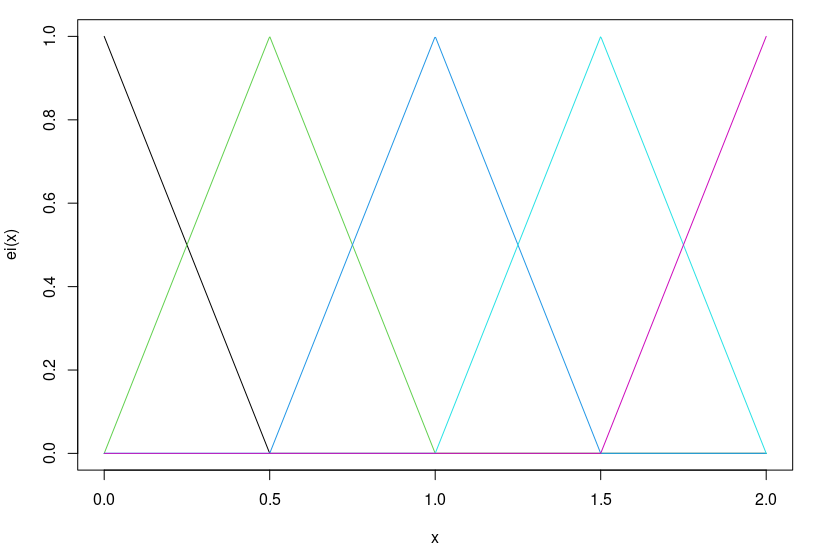
\includegraphics[width=0.7\textwidth]{img/base_functions.png}
    \caption{Wykres funkcji bazowych \( e_i(x) \) dla \( n = 4 \).}
\end{figure}

\begin{figure}[h]
    \centering
    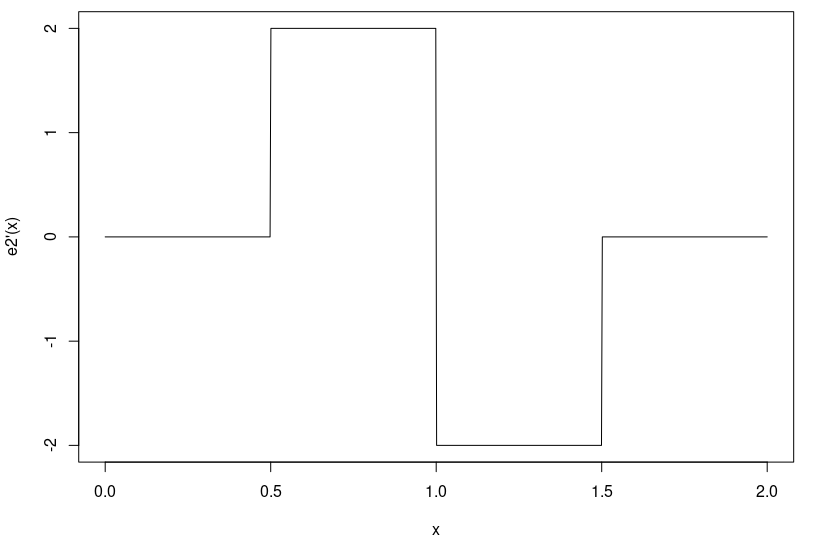
\includegraphics[width=0.7\textwidth]{img/derivative.png}
    \caption{Wykres pochodnej funkcji bazowej \( e_2(x) \) dla \( n = 4 \).}
\end{figure}

\cleardoublepage
\section{Rozwiązanie równania}

Biorąc pod uwagę określony zerowy warunek Dirichleta na brzegu \( \Omega \) w punkcie \( x = 2 \), pomijamy n-tą funkcję bazową. Poszukiwaną funkcję \( u \) będziemy przybliżać przy użyciu kombinacji liniowej funkcji bazowych.

\[
    u(x) \approx \sum_{i=0}^{n - 1} u_ie_i(x)
\]

Nieznanne współczynniki \( u_i \) obliczamy rozwiązując następujący układ równań.


\[
    \begin{cases}
        u_0B(e_0, e_0) + u_1B(e_1, e_0) + &\hdots + u_{n-1}B(e_{n-1}, e_0) = L(e_0) \\
        u_1B(e_0, e_1) + u_1B(e_1, e_1) + &\hdots + u_{n-1}B(e_{n-1}, e_1) = L(e_1) \\
        u_2B(e_0, e_2) + u_1B(e_1, e_2) + &\hdots + u_{n-1}B(e_{n-1}, e_2) = L(e_2) \\

        &\vdots \\
        
        u_{n-1}B(e_0, e_{n-1}) + u_1B(e_1, e_{n-1}) + &\hdots + u_{n-1}B(e_{n-1}, e_{n-1}) = L(e_{n-1}) \\
         
    \end{cases}
\]


Macierzowo:

\[
    \begin{bmatrix}
        B(e_0, e_0) & B(e_1, e_0) & \cdots & B(e_{n-1}, e_0) \\
        B(e_0, e_1) & B(e_1, e_1) & \cdots & B(e_{n-1}, e_1) \\
        \vdots & \vdots & \ddots & \vdots\\
        B(e_0, e_{n-1}) & B(e_1, e_{n-1}) & \cdots & B(e_{n-1}, e_{n-1}) \\
    \end{bmatrix}
    \begin{bmatrix}
        u_0\\u_1\\ \vdots\\u_{n-1}
    \end{bmatrix}
    =\begin{bmatrix}
        L(e_0)\\L(e_1)\\ \vdots\\L(e_{n-1})
    \end{bmatrix}
\]

Po wyliczeniu współczynników \( u_i \) otrzymujemy następujący wykres szukanej funkcji \( u(x) \).

\begin{figure}[h]
    \centering
    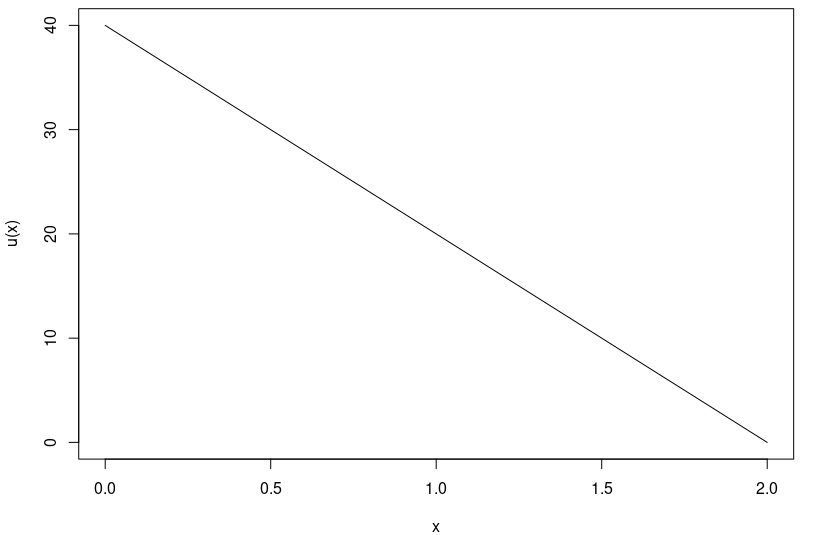
\includegraphics[width=0.7\textwidth]{img/solution.png}
    \caption{Wykres funkcji \( u(x) \) dla \( n = 100 \).}
\end{figure}


\end{document}